\section{Scope of reproducibility}



% In this section, I think the focus should be on "what are the central claims of the original paper that we hope to verify".

% Example of their claims:
% - (For the back-propagation till input space) When purturbing input features, changes in p_t (the softmax output) and accuracy match each other, whilst changes in y_t (the logits output) do not.
% - (For back-prop to input space) Weighted contrastive explanation is better at capturing the most important features.
% ...

% I'd like to structure this section as follows:
% - The central claims of the original paper that you verify (list them so that it is easy for the reviewer to check that you indeed verified the claims)
% - Additional experiments you did to test the generalizability of the proposed method, e.g.
% 	- XGradCAM
% 	- ViT with GradCAM and rollout 		w/ and w/o contrastive


\label{Contributions}
The claims of the original paper we seek to verify are:
\begin{itemize}
    \item \textbf{Claim 1:} When perturbing input features according to the original paper's weighted contrastive explanation, changes in the softmax output $p_t$ and accuracy match each other, whilst changes in the logit $y_t$ do not for target class $t$.
    \label{claim1}
    \label{claim2}
    \item \textbf{Claim 2:} The original paper's weighted contrastive explanation when coupled with a visualization method such as GradCAM highlights the most crucial areas for classification when the model classifies between several dominant classes.
    \label{claim3}
    \item \textbf{Claim 3:} The original paper's weighted contrastive explanation should be able to be easily applied to other back-propagation-based explanation methods by back-propagating from the softmax output $p_t$ rather than the logit $y_t$.
\end{itemize}

In order to evaluate the above claims and thus test the reproducibility of the paper we replicated the steps described in section \textit{5 Experiments} of the original paper for a subset of the models and datasets used in the original paper. We thus made our own experiments using our own code. The results of these experiments were then compared with those of the paper in order to find if they were consistent. We furthermore test the generalizability of the paper by applying the contrastive explanation method shown in the original paper using XGradCAM \citep{xgradcam}, FullGrad \citep{srinivasFullgradientRepresentationNeural2019}, and Vision Transformers \citep{visual-transformer}.



\subsection{XGradCAM and FullGrad}
\label{SectionXGradCAM}
As an attempt to test the paper's contrastive method's generalization capability additional back-propagation methods in the form of modified versions of XGradCAM \citep{xgradcam} and FullGrad \citep{srinivasFullgradientRepresentationNeural2019} were used. 

The modified version of XGradCAM removes ReLU, as in the original paper, and as a consequence uses the absolute values in the feature map sum when normalizing rather than only the sum. This gives the following explanation $\pmb{\phi}^t(\pmb{x})_y$ when back-propagating from the logit $y_t$ with the target feature map layer $\pmb{a}$ with $k \in K$ feature maps:

\begin{equation}
    \pmb{\phi}^t(\pmb{x})_y = \sum_{k}\left(\sum_{i,j} \frac{a_{ij}^k}{\|\pmb{a}^k\|_1} \frac{\partial y_t}{\partial a_{ij}^k}\right)\pmb{a}^k %= \sum_{k} \frac{\pmb{a}^k \cdot \nabla{\pmb{a}^k} y_t}{\|\pmb{a}^k\|_1}  \pmb{a}^k
\end{equation}

A weighted contrastive version, $\pmb{\phi}^t(\pmb{x})_{\textnormal{weighted}}$ as described in the original paper, of XGradCAM can be obtained by propagating from the softmax neuron $p_t$ and can be proven as follows using notation $[c]$ for all classes:

\begin{equation}
    \pmb{\phi}^t(\pmb{x})_p = \sum_{k}\left(\sum_{i,j} \frac{a_{ij}^k}{\|\pmb{a}^k\|_1} \sum_{s \in [c]}\left( \frac{\partial p_t}{\partial y_s}\frac{\partial y_s}{\partial a_{ij}^k}\right)\right)\pmb{a}^k = \sum_{s \in [c]} \frac{\partial p_t}{\partial y_s} \pmb{\phi}^s(\pmb{x})_y \propto \pmb{\phi}^t(\pmb{x})_{\textnormal{weighted}}
\end{equation}

The modified version of FullGrad changes the post-processing operations indicated by $\psi$ in \citep{srinivasFullgradientRepresentationNeural2019} by removing the abs function in order to be linear and therefore allow negative and positive values in the produced saliency map. This allows us to generate a contrastive weighted version by back-propagating from the target softmax neuron $p_t$ in but also heavily alters the method. 

\subsection{Vision Transformers}
In order to test how differences in architecture affect the results we modified two sets of explanation methods, GradCAM and and Gradient-weighted attention rollout \citep{blog-grad-rollout}, and tested them together with the \texttt{vit\_b\_16} model as first described in \citet{visual-transformer}. This model works by dividing the image into 16x16 patches, interpreting each patch of the image as a token. The information in these layers is then propagated throughout the network using a self-attention mechanism. Unlike standard convolutional neural network (CNN) architectures, spatial coherence is not guaranteed through the network, and information is easily mixed with some layers containing little to no spatial coherence.


% We have implemented the weighted contrastive method together with the \texttt{vit\_b\_16} model of the Vision Transformer architecture on a subset of the imagenet dataset. We find that the method is applicable with expected results. Though, due to the weaker spatial relationship between the input image and activations in transformers %https://arxiv.org/pdf/2005.00928.pdf
% we get significantly less "object-focused" explanations as seen in figure \ref{fig:vit-gradcam}. Therefore, we have also extended the explanation to gradient-weighted attention rollout - which is a  an explanation method based on the weighted sum of all attention layers - where the weights are determined by the gradient with regards to a target class, or in our case target softmax.

% Proof that this is correct?

% \subsubsection{Visual transformer: Contrastive GradCAM}
% In order to adapt GradCAM to Vision Transformer models, tokens are reimagined as the spatially coherent nodes in standard CNN models, with the tokens' features as channels. This results in a 16x16 explanation map after taking the mean of the channels in standard GradCAM fashion, these explanations are later upsampled to the original image's size. This method has been proposed and implemented in \cite{gradcam-vit}.

% In order to adapt the method to the contrastive version all ReLU operations have been removed and the gradients are calculated from the softmax output instead of the logits. 

% Due to the mixing of information during self-attention, most explanation maps produce qualitatively bad results, not highlighting the important parts of the image to our eyes. The layers in figure \ref{fig:vit-gradcam} have been explicitly selected because they gave good results, explanations in regard to other layers do not produce spatially coherent results.

% We find that the contrastive explanations with regards to the softmax do not have a significant effect on the results. We also observe that the explanation is often dominated by the explanation of the dominating class, if images are not selected to have similar probabilities for the top elements then there is usually no visual difference between doing a softmax GradCAM and a standard GradCAM without ReLU.


% \subsubsection{Visual Transformer: Contrastive Gradient-weighted attention rollout}
% Attention rollout is an explanation method proposed by the authors of \cite{visual-transformer} and further researched in \cite{Quantifying-Attention-Flow}. Here, attention is propagated throughout the network from layer to layer towards the input neurons by multiplying the attention. This method has later been further developed in order to weight explanations with regards to their gradients \cite{blog-grad-rollout} \cite{Chefer2020Dec}. 

% In order to adapt the method to the corresponding contrastive method, all ReLU operations have been removed and the gradient is calculated from the softmax output instead of the logits.

% This explanation is significantly more accurate to the perceived localization of the image. However, the contrastive method with regards to the softmax does not seem to significantly impact the explanation compared to the contrastive one.

% \begin{figure}[t!]
\tiny
\centering

%\begin{minipage}[b]{0.48\textwidth}
\resizebox{\textwidth}{!}{\
\begin{subfigure}{.5\textwidth}
\begin{tabular}
{ 
c@{\hspace{0.09cm}} c@{\hspace{0.09cm}} c@{\hspace{0.09cm}} c@{\hspace{0.09cm}} c@{\hspace{0.09cm}}}

    % & \textbf{Original} & \text{\textbf{Standard} \\ \textbf{GradCAM}} & \textbf{GradCAM}  \textbf{wo/ ReLU} & \textbf{Contrastive} \textbf{GradCAM} \\
    & \thead{Original} & \thead{Standard \\ GradCAM} & \thead{GradCAM \\ w/o ReLU} & \thead{Contrastive \\ GradCAM} \\
    
    \vspace{0.09cm}
    % $\vcenter{\hbox{Ice Cream}}$ &
    % \thead{Ice-\\cream \\ \texttt{p=0.30}} &
    $\vcenter{\hbox{\shortstack{\textbf{Ice} \textbf{cream} \\ p=0.30}}}$ &
    $\vcenter{\hbox{\includegraphics[width = \myfigurewidth\textwidth]{figures/vit-figures/icecream_l10_gradcam/original.jpg}}}$ &
    $\vcenter{\hbox{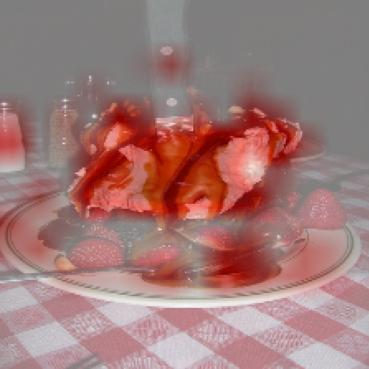
\includegraphics[width = \myfigurewidth\textwidth]{figures/vit-figures/icecream_l10_gradcam/standard_cam_w_relu.jpg}}}$ &
    $\vcenter{\hbox{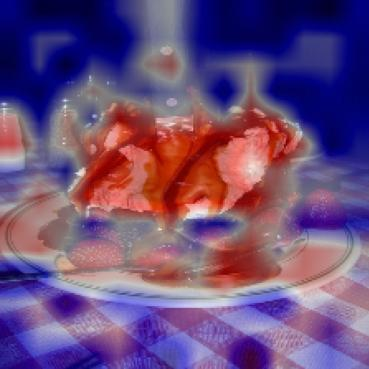
\includegraphics[width = \myfigurewidth\textwidth]{figures/vit-figures/icecream_l10_gradcam/standard_cam.jpg}}}$ &
    $\vcenter{\hbox{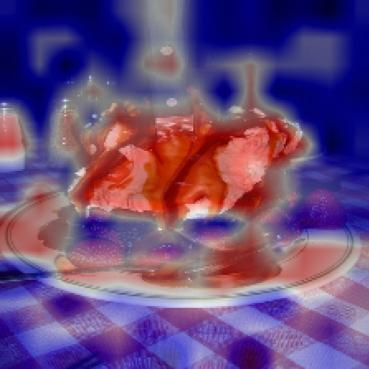
\includegraphics[width = \myfigurewidth\textwidth]{figures/vit-figures/icecream_l10_gradcam/contrastive_cam.jpg}}}$ \\

    \vspace{0.09cm}
    % \thead{Chocolate \\ Sauce} &
    $\vcenter{\hbox{\shortstack{\textbf{Chocolate} \\ \textbf{sauce} \\ p=0.30}}}$ &
    $\vcenter{\hbox{\includegraphics[width = \myfigurewidth\textwidth]{figures/vit-figures/chocolate_sauce_l10_gradcam/original.jpg}}}$ &
    $\vcenter{\hbox{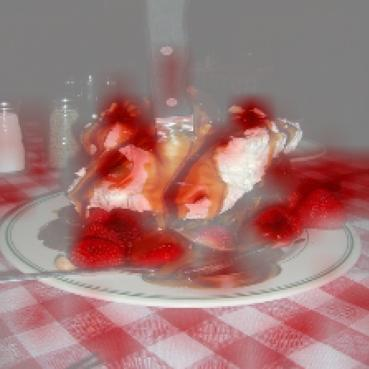
\includegraphics[width = \myfigurewidth\textwidth]{figures/vit-figures/chocolate_sauce_l10_gradcam/standard_cam_w_relu.jpg}}}$ &
    $\vcenter{\hbox{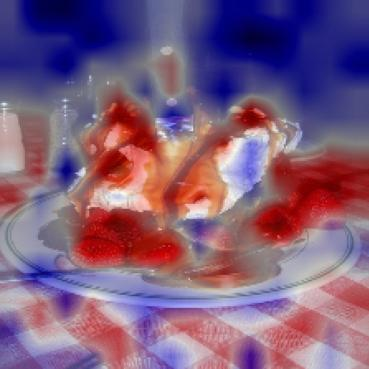
\includegraphics[width = \myfigurewidth\textwidth]{figures/vit-figures/chocolate_sauce_l10_gradcam/standard_cam.jpg}}}$ &
    $\vcenter{\hbox{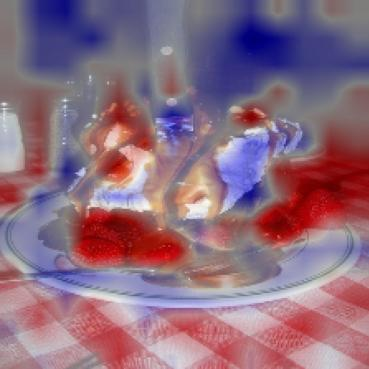
\includegraphics[width = \myfigurewidth\textwidth]{figures/vit-figures/chocolate_sauce_l10_gradcam/contrastive_cam.jpg}}}$ \\

    \vspace{0.09cm}
    % $\vcenter{\hbox{Digital Watch}}$ &
    % \thead{Digital \\ Watch} &
    $\vcenter{\hbox{\shortstack{\textbf{Digital} \\ \textbf{watch} \\ p=0.32}}}$ &
    $\vcenter{\hbox{\includegraphics[width = \myfigurewidth\textwidth]{figures/vit-figures/digital_watch_l10_gradcam/original.jpg}}}$ &
    $\vcenter{\hbox{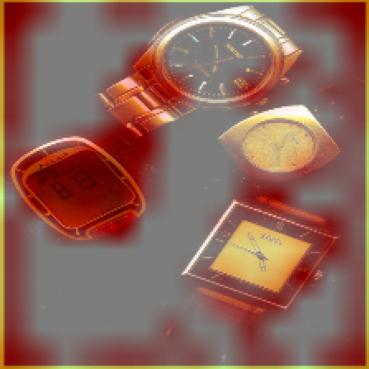
\includegraphics[width = \myfigurewidth\textwidth]{figures/vit-figures/digital_watch_l10_gradcam/standard_cam_w_relu.jpg}}}$ &
    $\vcenter{\hbox{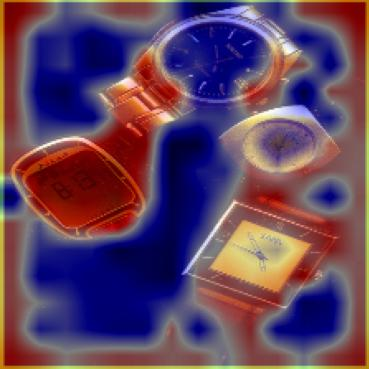
\includegraphics[width = \myfigurewidth\textwidth]{figures/vit-figures/digital_watch_l10_gradcam/standard_cam.jpg}}}$ &
    $\vcenter{\hbox{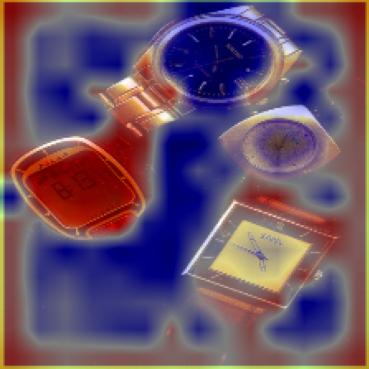
\includegraphics[width = \myfigurewidth\textwidth]{figures/vit-figures/digital_watch_l10_gradcam/contrastive_cam.jpg}}}$ \\

    \vspace{0.09cm}
    % $\vcenter{\hbox{Stopwatch}}$ &
    % \thead{Stop-\\watch} &
    $\vcenter{\hbox{\shortstack{\textbf{Stopwatch} \\ p=0.32}}}$ &
    $\vcenter{\hbox{\includegraphics[width = \myfigurewidth\textwidth]{figures/vit-figures/stopwatch_l10_gradcam/original.jpg}}}$ &
    $\vcenter{\hbox{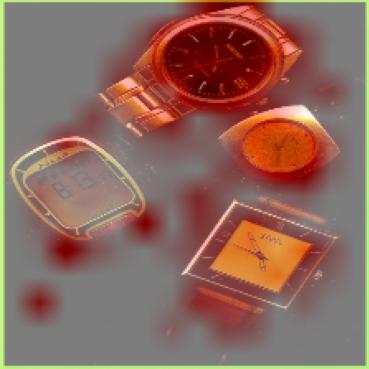
\includegraphics[width = \myfigurewidth\textwidth]{figures/vit-figures/stopwatch_l10_gradcam/standard_cam_w_relu.jpg}}}$ &
    $\vcenter{\hbox{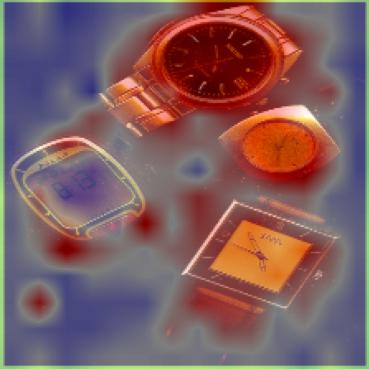
\includegraphics[width = \myfigurewidth\textwidth]{figures/vit-figures/stopwatch_l10_gradcam/standard_cam.jpg}}}$ &
    $\vcenter{\hbox{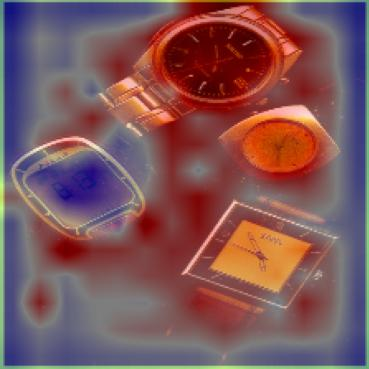
\includegraphics[width = \myfigurewidth\textwidth]{figures/vit-figures/stopwatch_l10_gradcam/contrastive_cam.jpg}}}$ \\  

\end{tabular}
\caption{} \label{t:}
\label{fig:vit-gradcam}
\end{subfigure}

\begin{subfigure}{.5\textwidth}
\begin{tabular}
{ 
c@{\hspace{0.09cm}} c@{\hspace{0.09cm}} c@{\hspace{0.09cm}} c@{\hspace{0.09cm}} c@{\hspace{0.09cm}}}
    & \thead{Original} & \thead{Gradient-\\weighted \\ Attention \\ Rollout} & \thead{Gradient-\\ weighted \\ Attention \\ Rollout \\ w/o ReLU} & \thead{Contrastive \\ Gradient-\\weighted \\ Attention \\ Rollout} \\
    
    \vspace{0.09cm}
    $\vcenter{\hbox{\shortstack{\textbf{Ice} \textbf{cream} \\ p=0.30}}}$ &
    $\vcenter{\hbox{\includegraphics[width = \myfigurewidth\textwidth]{figures/vit-figures/attention_rollout/icecream/original.png}}}$ &
    $\vcenter{\hbox{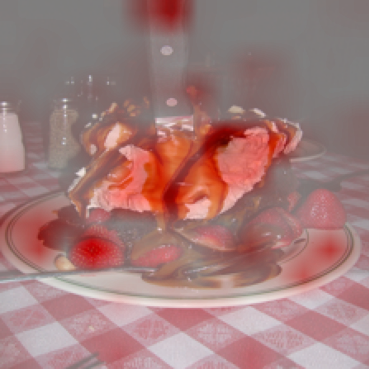
\includegraphics[width = \myfigurewidth\textwidth]{figures/vit-figures/attention_rollout/icecream/standard.png}}}$ &
    $\vcenter{\hbox{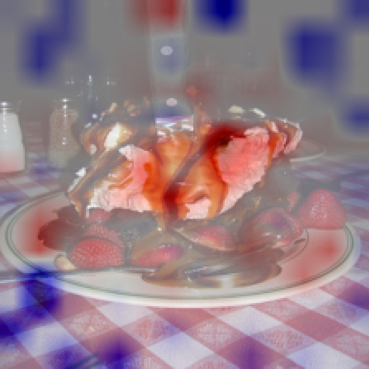
\includegraphics[width = \myfigurewidth\textwidth]{figures/vit-figures/attention_rollout/icecream/standard_contrastive.png}}}$ &
    $\vcenter{\hbox{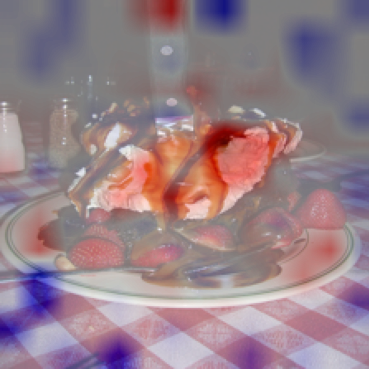
\includegraphics[width = \myfigurewidth\textwidth]{figures/vit-figures/attention_rollout/icecream/contrastive.png}}}$ \\

    \vspace{0.09cm}
    $\vcenter{\hbox{\shortstack{\textbf{Chocolate} \\ \textbf{sauce} \\ p=0.30}}}$ &
    $\vcenter{\hbox{\includegraphics[width = \myfigurewidth\textwidth]{figures/vit-figures/attention_rollout/chocolate/original.png}}}$ &
    $\vcenter{\hbox{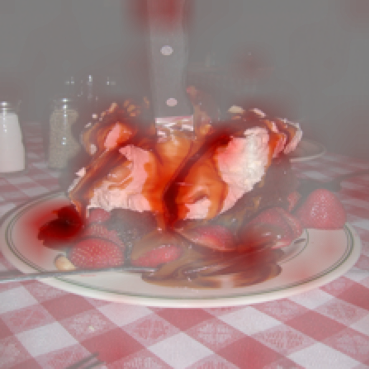
\includegraphics[width = \myfigurewidth\textwidth]{figures/vit-figures/attention_rollout/chocolate/standard.png}}}$ &
    $\vcenter{\hbox{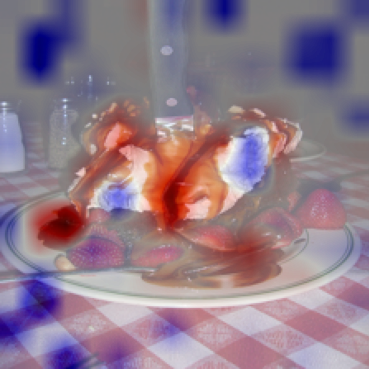
\includegraphics[width = \myfigurewidth\textwidth]{figures/vit-figures/attention_rollout/chocolate/standard_contrastive.png}}}$ &
    $\vcenter{\hbox{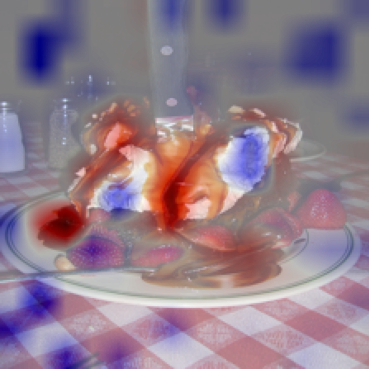
\includegraphics[width = \myfigurewidth\textwidth]{figures/vit-figures/attention_rollout/chocolate/contrastive.png}}}$ \\

    \vspace{0.09cm}
    $\vcenter{\hbox{\shortstack{\textbf{Digital} \\ \textbf{watch} \\ p=0.32}}}$ &
    $\vcenter{\hbox{\includegraphics[width = \myfigurewidth\textwidth]{figures/vit-figures/attention_rollout/digital/original.png}}}$ &
    $\vcenter{\hbox{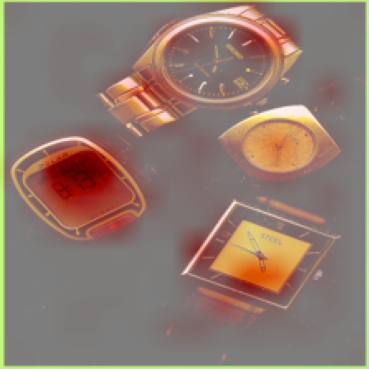
\includegraphics[width = \myfigurewidth\textwidth]{figures/vit-figures/attention_rollout/digital/standard.png}}}$ &
    $\vcenter{\hbox{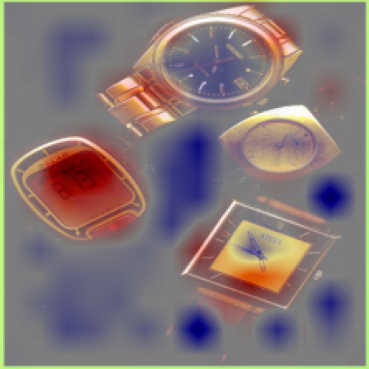
\includegraphics[width = \myfigurewidth\textwidth]{figures/vit-figures/attention_rollout/digital/standard_contrastive.png}}}$ &
    $\vcenter{\hbox{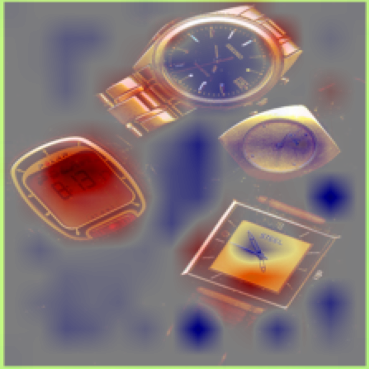
\includegraphics[width = \myfigurewidth\textwidth]{figures/vit-figures/attention_rollout/digital/contrastive.png}}}$ \\

    \vspace{0.09cm}
    $\vcenter{\hbox{\shortstack{\textbf{Stopwatch} \\ p=0.32}}}$ &
    $\vcenter{\hbox{\includegraphics[width = \myfigurewidth\textwidth]{figures/vit-figures/attention_rollout/stopwatch/original.png}}}$ &
    $\vcenter{\hbox{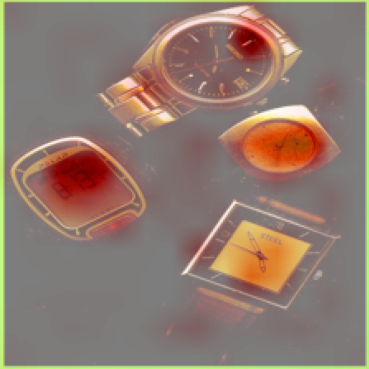
\includegraphics[width = \myfigurewidth\textwidth]{figures/vit-figures/attention_rollout/stopwatch/standard.png}}}$ &
    $\vcenter{\hbox{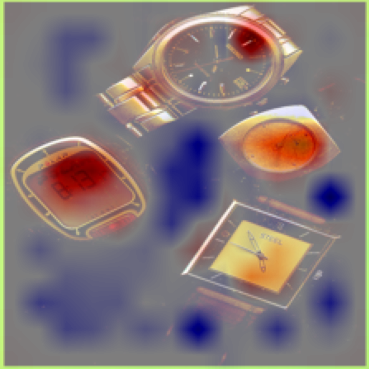
\includegraphics[width = \myfigurewidth\textwidth]{figures/vit-figures/attention_rollout/stopwatch/standard_contrastive.png}}}$ &
    $\vcenter{\hbox{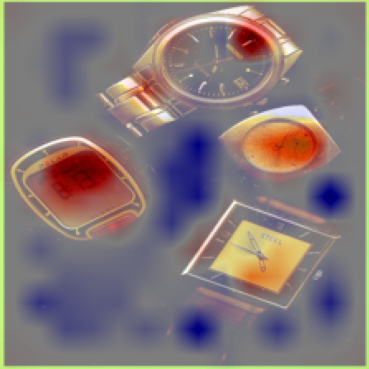
\includegraphics[width = \myfigurewidth\textwidth]{figures/vit-figures/attention_rollout/stopwatch/contrastive.png}}}$ \\

\end{tabular}
\caption{} \label{t:}
\end{subfigure}
}

\caption{Comparison between proposed ViT explanations for a pre-trained ImageNet model. In (a) a comparison between GradCAM, GradCAM without ReLU, and Contrastive GradCAM is considered. In (b) a comparison between Gradient-weighted Attention rollout (GWAR) of the standard, without ReLU, and contrastive variant is considered. Red sections are considered areas with high explainability. To adapt the method to the contrastive version all ReLU operations were removed and the gradients were calculated from the softmax output instead of the logits.} \label{t:}
\end{figure}

